\documentclass[]{article}
\usepackage{lmodern}
\usepackage{amssymb,amsmath}
\usepackage{ifxetex,ifluatex}
\usepackage{fixltx2e} % provides \textsubscript
\ifnum 0\ifxetex 1\fi\ifluatex 1\fi=0 % if pdftex
  \usepackage[T1]{fontenc}
  \usepackage[utf8]{inputenc}
\else % if luatex or xelatex
  \ifxetex
    \usepackage{mathspec}
  \else
    \usepackage{fontspec}
  \fi
  \defaultfontfeatures{Ligatures=TeX,Scale=MatchLowercase}
\fi
% use upquote if available, for straight quotes in verbatim environments
\IfFileExists{upquote.sty}{\usepackage{upquote}}{}
% use microtype if available
\IfFileExists{microtype.sty}{%
\usepackage{microtype}
\UseMicrotypeSet[protrusion]{basicmath} % disable protrusion for tt fonts
}{}
\usepackage[margin=1in]{geometry}
\usepackage{hyperref}
\hypersetup{unicode=true,
            pdftitle={week2 project},
            pdfauthor={hongyuatcufe},
            pdfborder={0 0 0},
            breaklinks=true}
\urlstyle{same}  % don't use monospace font for urls
\usepackage{color}
\usepackage{fancyvrb}
\newcommand{\VerbBar}{|}
\newcommand{\VERB}{\Verb[commandchars=\\\{\}]}
\DefineVerbatimEnvironment{Highlighting}{Verbatim}{commandchars=\\\{\}}
% Add ',fontsize=\small' for more characters per line
\usepackage{framed}
\definecolor{shadecolor}{RGB}{248,248,248}
\newenvironment{Shaded}{\begin{snugshade}}{\end{snugshade}}
\newcommand{\AlertTok}[1]{\textcolor[rgb]{0.94,0.16,0.16}{#1}}
\newcommand{\AnnotationTok}[1]{\textcolor[rgb]{0.56,0.35,0.01}{\textbf{\textit{#1}}}}
\newcommand{\AttributeTok}[1]{\textcolor[rgb]{0.77,0.63,0.00}{#1}}
\newcommand{\BaseNTok}[1]{\textcolor[rgb]{0.00,0.00,0.81}{#1}}
\newcommand{\BuiltInTok}[1]{#1}
\newcommand{\CharTok}[1]{\textcolor[rgb]{0.31,0.60,0.02}{#1}}
\newcommand{\CommentTok}[1]{\textcolor[rgb]{0.56,0.35,0.01}{\textit{#1}}}
\newcommand{\CommentVarTok}[1]{\textcolor[rgb]{0.56,0.35,0.01}{\textbf{\textit{#1}}}}
\newcommand{\ConstantTok}[1]{\textcolor[rgb]{0.00,0.00,0.00}{#1}}
\newcommand{\ControlFlowTok}[1]{\textcolor[rgb]{0.13,0.29,0.53}{\textbf{#1}}}
\newcommand{\DataTypeTok}[1]{\textcolor[rgb]{0.13,0.29,0.53}{#1}}
\newcommand{\DecValTok}[1]{\textcolor[rgb]{0.00,0.00,0.81}{#1}}
\newcommand{\DocumentationTok}[1]{\textcolor[rgb]{0.56,0.35,0.01}{\textbf{\textit{#1}}}}
\newcommand{\ErrorTok}[1]{\textcolor[rgb]{0.64,0.00,0.00}{\textbf{#1}}}
\newcommand{\ExtensionTok}[1]{#1}
\newcommand{\FloatTok}[1]{\textcolor[rgb]{0.00,0.00,0.81}{#1}}
\newcommand{\FunctionTok}[1]{\textcolor[rgb]{0.00,0.00,0.00}{#1}}
\newcommand{\ImportTok}[1]{#1}
\newcommand{\InformationTok}[1]{\textcolor[rgb]{0.56,0.35,0.01}{\textbf{\textit{#1}}}}
\newcommand{\KeywordTok}[1]{\textcolor[rgb]{0.13,0.29,0.53}{\textbf{#1}}}
\newcommand{\NormalTok}[1]{#1}
\newcommand{\OperatorTok}[1]{\textcolor[rgb]{0.81,0.36,0.00}{\textbf{#1}}}
\newcommand{\OtherTok}[1]{\textcolor[rgb]{0.56,0.35,0.01}{#1}}
\newcommand{\PreprocessorTok}[1]{\textcolor[rgb]{0.56,0.35,0.01}{\textit{#1}}}
\newcommand{\RegionMarkerTok}[1]{#1}
\newcommand{\SpecialCharTok}[1]{\textcolor[rgb]{0.00,0.00,0.00}{#1}}
\newcommand{\SpecialStringTok}[1]{\textcolor[rgb]{0.31,0.60,0.02}{#1}}
\newcommand{\StringTok}[1]{\textcolor[rgb]{0.31,0.60,0.02}{#1}}
\newcommand{\VariableTok}[1]{\textcolor[rgb]{0.00,0.00,0.00}{#1}}
\newcommand{\VerbatimStringTok}[1]{\textcolor[rgb]{0.31,0.60,0.02}{#1}}
\newcommand{\WarningTok}[1]{\textcolor[rgb]{0.56,0.35,0.01}{\textbf{\textit{#1}}}}
\usepackage{graphicx,grffile}
\makeatletter
\def\maxwidth{\ifdim\Gin@nat@width>\linewidth\linewidth\else\Gin@nat@width\fi}
\def\maxheight{\ifdim\Gin@nat@height>\textheight\textheight\else\Gin@nat@height\fi}
\makeatother
% Scale images if necessary, so that they will not overflow the page
% margins by default, and it is still possible to overwrite the defaults
% using explicit options in \includegraphics[width, height, ...]{}
\setkeys{Gin}{width=\maxwidth,height=\maxheight,keepaspectratio}
\IfFileExists{parskip.sty}{%
\usepackage{parskip}
}{% else
\setlength{\parindent}{0pt}
\setlength{\parskip}{6pt plus 2pt minus 1pt}
}
\setlength{\emergencystretch}{3em}  % prevent overfull lines
\providecommand{\tightlist}{%
  \setlength{\itemsep}{0pt}\setlength{\parskip}{0pt}}
\setcounter{secnumdepth}{0}
% Redefines (sub)paragraphs to behave more like sections
\ifx\paragraph\undefined\else
\let\oldparagraph\paragraph
\renewcommand{\paragraph}[1]{\oldparagraph{#1}\mbox{}}
\fi
\ifx\subparagraph\undefined\else
\let\oldsubparagraph\subparagraph
\renewcommand{\subparagraph}[1]{\oldsubparagraph{#1}\mbox{}}
\fi

%%% Use protect on footnotes to avoid problems with footnotes in titles
\let\rmarkdownfootnote\footnote%
\def\footnote{\protect\rmarkdownfootnote}

%%% Change title format to be more compact
\usepackage{titling}

% Create subtitle command for use in maketitle
\providecommand{\subtitle}[1]{
  \posttitle{
    \begin{center}\large#1\end{center}
    }
}

\setlength{\droptitle}{-2em}

  \title{week2 project}
    \pretitle{\vspace{\droptitle}\centering\huge}
  \posttitle{\par}
    \author{hongyuatcufe}
    \preauthor{\centering\large\emph}
  \postauthor{\par}
      \predate{\centering\large\emph}
  \postdate{\par}
    \date{2022/2/2}


\begin{document}
\maketitle

\hypertarget{week2-project-by-hongyuatcufe}{%
\section{Week2 project by
hongyuatcufe}\label{week2-project-by-hongyuatcufe}}

\hypertarget{loading-and-preprocessing-the-data}{%
\subsection{1.Loading and preprocessing the
data}\label{loading-and-preprocessing-the-data}}

Read activity.csv file to variable activity.

\begin{Shaded}
\begin{Highlighting}[]
\NormalTok{activity}\OtherTok{=}\FunctionTok{read.csv}\NormalTok{(}\StringTok{\textquotesingle{}activity.csv\textquotesingle{}}\NormalTok{)}
\NormalTok{activity[[}\DecValTok{2}\NormalTok{]]}\OtherTok{=}\FunctionTok{as.Date}\NormalTok{(activity[[}\DecValTok{2}\NormalTok{]])}
\FunctionTok{head}\NormalTok{(activity)}
\end{Highlighting}
\end{Shaded}

\begin{verbatim}
##   steps       date interval
## 1    NA 2012-10-01        0
## 2    NA 2012-10-01        5
## 3    NA 2012-10-01       10
## 4    NA 2012-10-01       15
## 5    NA 2012-10-01       20
## 6    NA 2012-10-01       25
\end{verbatim}

\hypertarget{caculate-the-mean-total-number-of-steps-taken-per-day}{%
\subsection{2.Caculate the mean total number of steps taken per
day}\label{caculate-the-mean-total-number-of-steps-taken-per-day}}

Calculate the total number of steps taken per day

\begin{Shaded}
\begin{Highlighting}[]
\FunctionTok{library}\NormalTok{(dplyr)}

\NormalTok{steps\_per\_day }\OtherTok{\textless{}{-}}\NormalTok{ activity }\SpecialCharTok{\%\textgreater{}\%}
  \FunctionTok{group\_by}\NormalTok{(date) }\SpecialCharTok{\%\textgreater{}\%}
  \FunctionTok{summarise}\NormalTok{(}\AttributeTok{steps=}\FunctionTok{sum}\NormalTok{(steps,}\AttributeTok{na.rm=}\ConstantTok{TRUE}\NormalTok{))}

\FunctionTok{head}\NormalTok{(steps\_per\_day)}
\end{Highlighting}
\end{Shaded}

\begin{verbatim}
## # A tibble: 6 x 2
##   date       steps
##   <date>     <int>
## 1 2012-10-01     0
## 2 2012-10-02   126
## 3 2012-10-03 11352
## 4 2012-10-04 12116
## 5 2012-10-05 13294
## 6 2012-10-06 15420
\end{verbatim}

Make a histogram of the total number of steps taken each day

\begin{Shaded}
\begin{Highlighting}[]
\CommentTok{\# set breaks to 10 to make the histogram show more details}
\FunctionTok{hist}\NormalTok{(steps\_per\_day}\SpecialCharTok{$}\NormalTok{steps,}\AttributeTok{breaks=}\DecValTok{10}\NormalTok{)}
\end{Highlighting}
\end{Shaded}

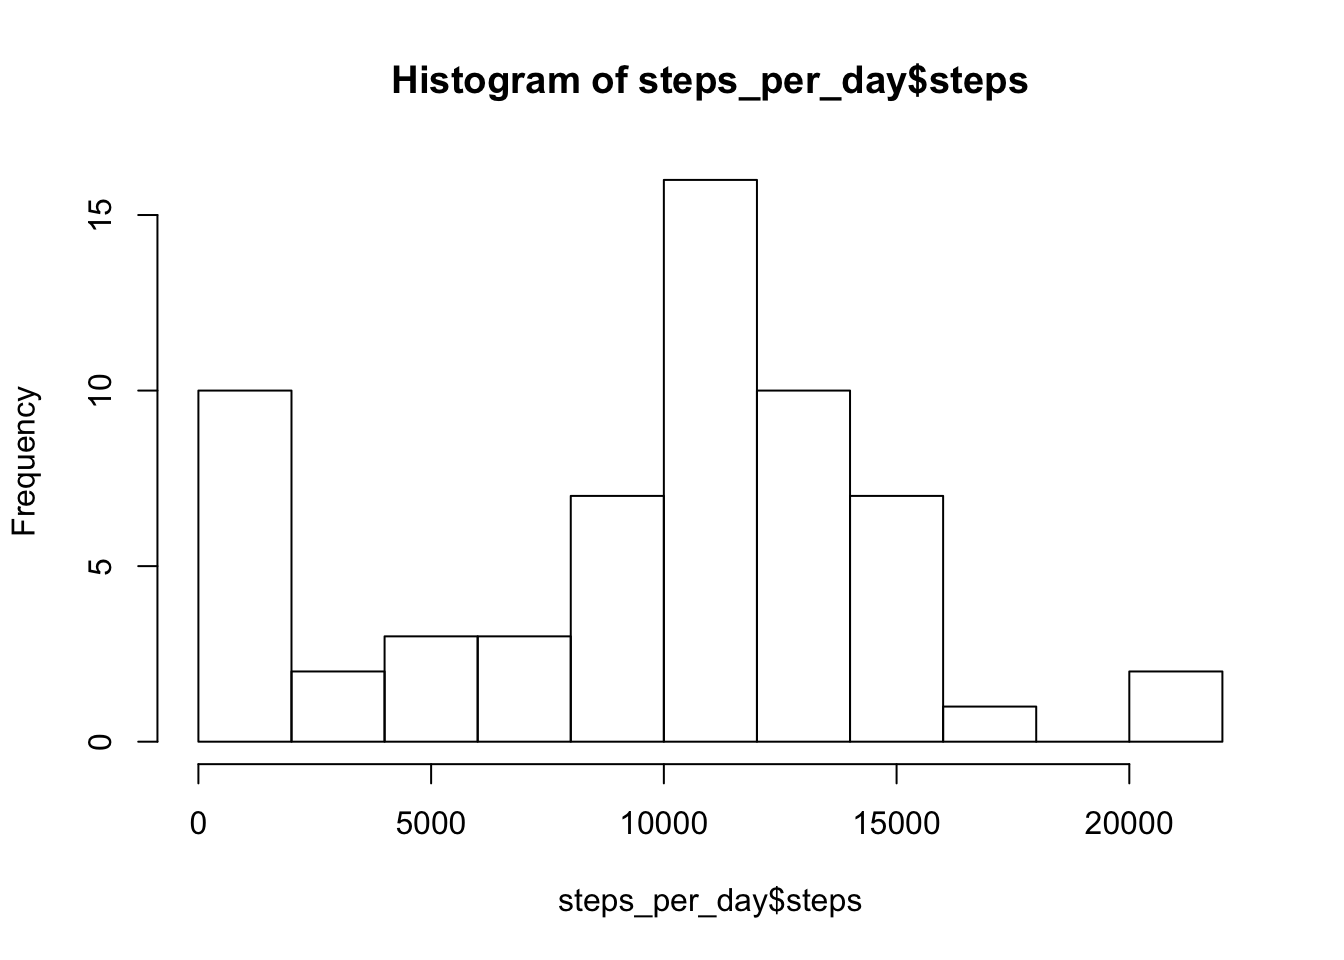
\includegraphics{PA1_template_files/figure-latex/unnamed-chunk-3-1.pdf}

Calculate and report the mean and median of the total number of steps
taken per day

\begin{Shaded}
\begin{Highlighting}[]
\CommentTok{\# Caculate the mean and median of steps}
\NormalTok{steps\_mean}\OtherTok{=}\FunctionTok{mean}\NormalTok{(steps\_per\_day}\SpecialCharTok{$}\NormalTok{steps)}
\NormalTok{steps\_median}\OtherTok{=}\FunctionTok{median}\NormalTok{(steps\_per\_day}\SpecialCharTok{$}\NormalTok{steps)}
\CommentTok{\# print the results}
\FunctionTok{print}\NormalTok{(}\FunctionTok{paste}\NormalTok{(}\StringTok{\textquotesingle{}The mean of steps per day is\textquotesingle{}}\NormalTok{,}\FunctionTok{round}\NormalTok{(steps\_mean,}\DecValTok{2}\NormalTok{),}\StringTok{\textquotesingle{}and\textquotesingle{}}\NormalTok{,}
      \FunctionTok{paste}\NormalTok{(}\StringTok{"The median of steps per day is"}\NormalTok{,steps\_median)))}
\end{Highlighting}
\end{Shaded}

\begin{verbatim}
## [1] "The mean of steps per day is 9354.23 and The median of steps per day is 10395"
\end{verbatim}

\hypertarget{caculate-the-average-daily-activity-pattern}{%
\subsection{3.Caculate the average daily activity
pattern}\label{caculate-the-average-daily-activity-pattern}}

time series plot (i.e.~type = ``l'') of the 5-minute interval (x-axis)
and the average number of steps taken, averaged across all days (y-axis)

\begin{Shaded}
\begin{Highlighting}[]
\NormalTok{steps\_per\_interval }\OtherTok{\textless{}{-}}\NormalTok{ activity }\SpecialCharTok{\%\textgreater{}\%}
  \FunctionTok{group\_by}\NormalTok{(interval) }\SpecialCharTok{\%\textgreater{}\%}
  \FunctionTok{summarise}\NormalTok{(}\AttributeTok{steps=}\FunctionTok{mean}\NormalTok{(steps,}\AttributeTok{na.rm=}\ConstantTok{TRUE}\NormalTok{))}

\FunctionTok{plot}\NormalTok{(steps\_per\_interval,}\AttributeTok{type=}\StringTok{\textquotesingle{}l\textquotesingle{}}\NormalTok{)}
\end{Highlighting}
\end{Shaded}

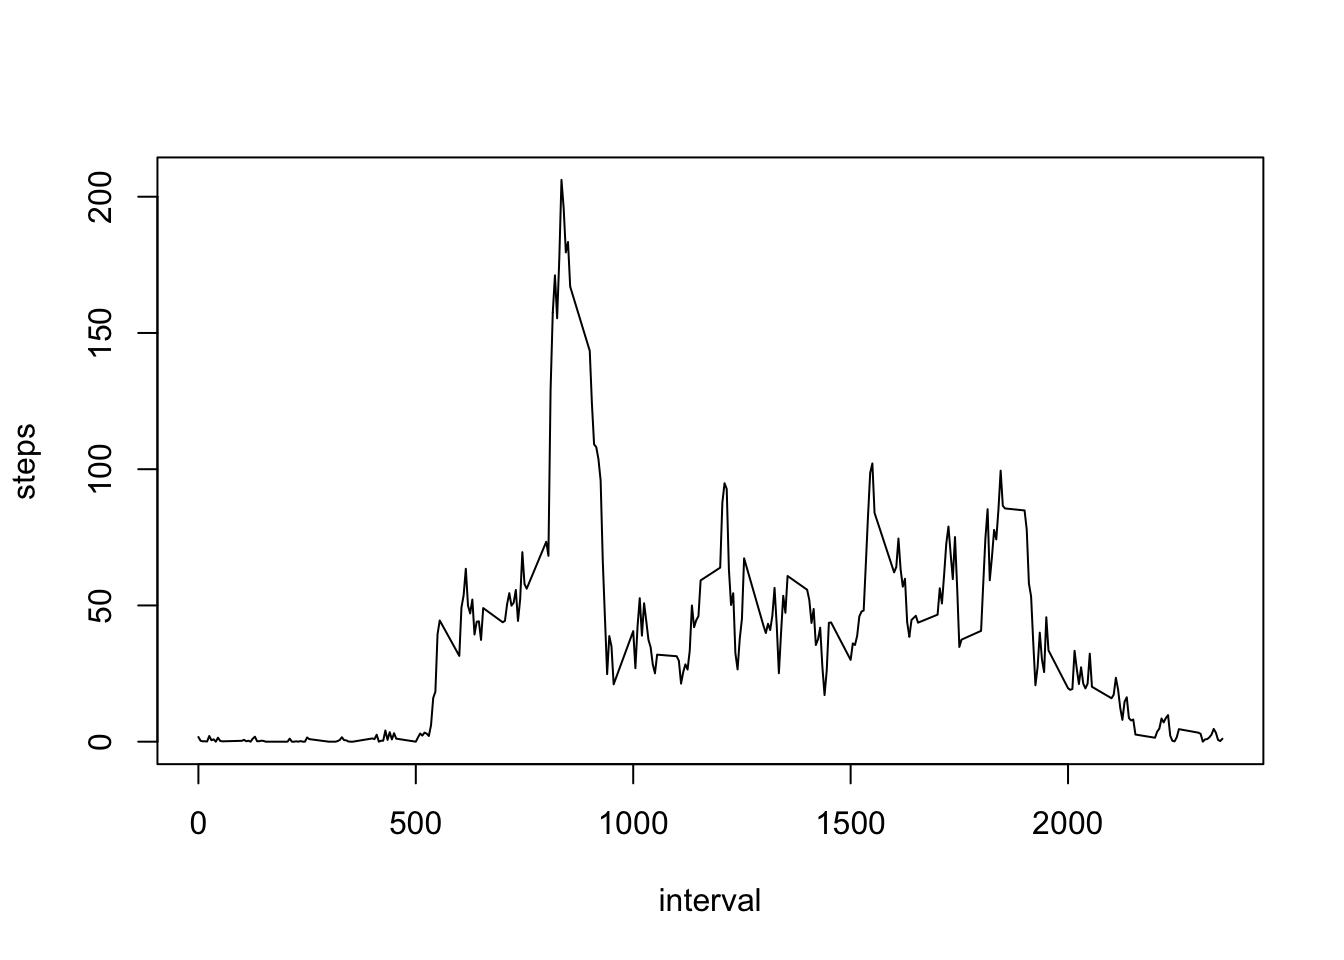
\includegraphics{PA1_template_files/figure-latex/unnamed-chunk-5-1.pdf}

\begin{Shaded}
\begin{Highlighting}[]
\NormalTok{max\_step\_interval}\OtherTok{=}\NormalTok{steps\_per\_interval[steps\_per\_interval}\SpecialCharTok{$}\NormalTok{steps}\SpecialCharTok{==}\FunctionTok{max}\NormalTok{(steps\_per\_interval}\SpecialCharTok{$}\NormalTok{steps),}\StringTok{\textquotesingle{}interval\textquotesingle{}}\NormalTok{]}
\FunctionTok{print}\NormalTok{(}\FunctionTok{paste}\NormalTok{(}\StringTok{\textquotesingle{}The max of the average number of steps taken occur in interval\textquotesingle{}}\NormalTok{, max\_step\_interval))}
\end{Highlighting}
\end{Shaded}

\begin{verbatim}
## [1] "The max of the average number of steps taken occur in interval 835"
\end{verbatim}

The max of the average number of steps taken occur at 8:35 AM.

\hypertarget{imputing-missing-values}{%
\subsection{Imputing missing values}\label{imputing-missing-values}}

Calculate and report the total number of missing values in the dataset
(i.e.~the total number of rows with NAs)

\begin{Shaded}
\begin{Highlighting}[]
\NormalTok{steps\_missing}\OtherTok{=}\FunctionTok{sum}\NormalTok{(}\FunctionTok{is.na}\NormalTok{(activity}\SpecialCharTok{$}\NormalTok{steps))}
\FunctionTok{print}\NormalTok{(}\FunctionTok{paste}\NormalTok{(}\StringTok{\textquotesingle{}The total number of missing values in the dataset is\textquotesingle{}}\NormalTok{,steps\_missing))}
\end{Highlighting}
\end{Shaded}

\begin{verbatim}
## [1] "The total number of missing values in the dataset is 2304"
\end{verbatim}


\end{document}
